\chapter{\ifproject%
      \ifenglish Experimentation and Results\else การทดลองและผลลัพธ์\fi
  \else%
      \ifenglish System Evaluation\else การประเมินระบบ\fi
  \fi}



\section{\ifenglish put the name here \else การสำรวจความคิดเห็นต่อเกมสยองขวัญ\fi}
จากผลสำรวจกลุ่มเป้าหมายทั้งหมด 47 คน ได้ผลสรุปดังนี้
\begin{itemize}
    \item สาเหตุที่ผู้เล่นนั้น ไม่สามารถเล่นเกมจนจบได้นั้น คือ อันดับ 1 ไม่มีเวลาเล่น คิดเป็น 74.5$\%$, อันดับ 2 ไม่มีคนเล่นด้วย คิดเป็น 53.2$\%$, และอันดับ 3 คู่ร่วม คือ เนื้อเรื่องไม่มีความน่าสนใจ และ มีเกมอื่นที่น่าสนใจมากกว่า คิดเป็น 18.3$\%$
    \item เกมแนวสยองขวัญควรมีอะไรบ้าง คือ อันดับ 1 มีฉากนองเลือด คิดเป็น 85.1$\%$, อันดับ 2 มีบรรยากาศที่ดูอึดอัด คิดเป็น 76.6$\%$, และอันดับ 3 ความมืด คิดเป็น 74.5$\%$
    \item สิ่งที่ไม่ถูกใจในเกมสยองขวัญคือ มีความยากในการเล่นสูงเกินไป มีความซ้ำซากจำเจ ต่อสู้กับผีไม่ได้ และมีฉาก jump scare มากเกินไป
\end{itemize}
\begin{figure}[h]
    \centering
    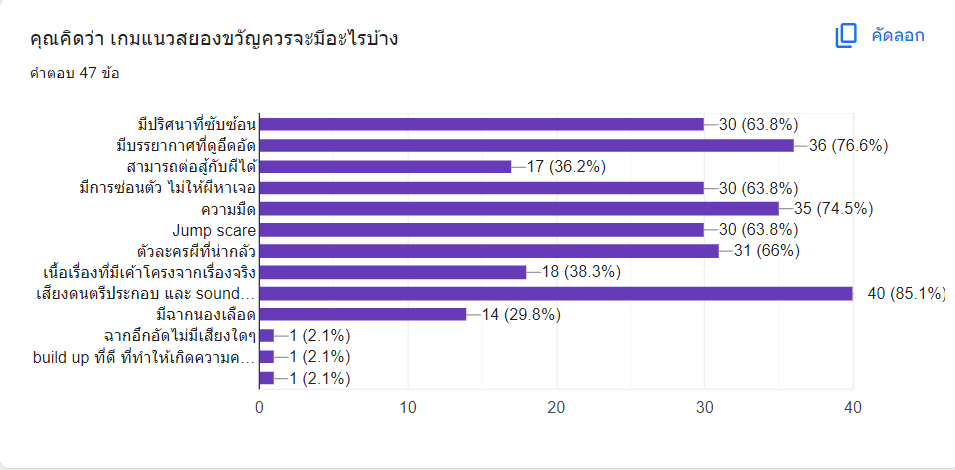
\includegraphics[width=\textwidth]{Images/Screenshot 2023-10-06 192027.png}
    \caption{ภาพผลสำรวจความคิดเห็นที่มีต่อเกมสยองขวัญ}\label{Empatize}
\end{figure}
\section{\ifenglish put the name here \else การวางแผนการประเมินผลสัมฤทธิ์ของโปรเจค\fi}
\begin{enumerate}
    \item นำ prototype มาทดสอบกับกลุ่มผู้ใช้งาน โดยให้เวลาในการทดสอบของแต่ละคน 15 นาที โดยใช้อุปกรณ์ที่เราได้จัดเตรียมไว้
    \item สอบถามปัญหา จากการใช้งาน prototype
    \item นำแบบทดสอบให้ทำ หลังการทดสอบ โดยมีเนื้อหาใจความดังนี้
    \begin{itemize}
        \item ท่านให้ความน่ากลัวของเกมนี้ อยู่ในระดับไหน 0-10 โดยที่ 0 คือ ไม่เห็นน่ากลัวเลย, 3 คือ น่ากลัวนิดๆหน่อยๆ, 5 คือ ก็น่ากลัวนะ, 7 คือ น่ากลัวมากๆ, และ 10 คือ จะน่ากลัวไปไหน
        \item ท่านให้ความสนุกอยู่ระดับ 0 - 10 โดยที่ 0 คือ ไม่สนุกเลย, 3 คือ สนุกนิดหน่อย, 5 คือ สนุกปานกลางๆ, 7 คือ สนุกมาก, และ 10 คือ สนุกที่สุด
        \item มีเนื้อเรื่องส่วนใด ที่ท่านชอบมากที่สุด อธิบาย
    \end{itemize}
\end{enumerate}